\chapter{Introduzione sulle tecniche di trasmissione}
\label{cha:intro}

 La comunicazione fra gli esseri umani è senzadubbio una delle abilità che hanno permesso all' uomo di evolversi. Sin dall'alba della civiltà l'uomo ha utilizzato la comunicazione per esprimere bisogni o intenzioni ai propri simili. La prima forma di comunicazione è stata senzadubbio quella verbale, metodo molto rapido ed efficace che però non garantisce la durata delle informazioni trasmesse. Altri metodi di comunicazione vennero sviluppati alcuni fra i più interessanti sono le nuvole di fumo che venivano utilizzate dagli indigeni d'america e più recentemente dai cinesi per comunicare lungo la grande muraglia cinese ed i tamburi utilizzati dalle tribù africane. La scrittura apparse circa 7000 anni fa favorendo l'inizio di un progresso che porterà l'uomo verso il ruolo centrale che ha ora sulla terra. Già nell'epoca della nascita di cristo l'uomo aveva instaurato una rete di comunicazione in forma scritta che interessava tutto il vecchio continente e lo collegava anche al mondo indiano ed orientale. Altri metodi un po' particolari vennero sfruttati prima dell' invenzione dell' elettricità come ad esempio i piccioni viaggiatori oppure l'utilizzo di una lingua formata da fischi fra le lunghe valli nelle isole dell'arcipelago delle Canarie.
Con la scoperta della corrente elettrica si è aperto per noi un nuovo mondo di possibilità fra le quali quella di trasferire immense quantità di informazioni velocemente e su lunghe distanze. Dapprima il telegrafo e poi il telefono fino ad arrivare alle trasmissioni analogiche seguite dall' avvento dell' era digitale. Nelle telecomunicazioni moderne per trasmettere si utilizza una portante (segnale elettrico oppure onda elettromagnetica) alla quale vengono aggiunte le informazioni secondo diverse tecniche dette anche modulazioni. Alcune principali modulazioni sono elencate e discusse in seguito.


\section{Modulazioni Analogiche}
\label{sec:context}

\begin{itemize}
   	\item \subsection{AM (amplitude modulation): } la modulazione in ampiezza è stata una delle prime modulazioni utilizzate grazie alla sua facilità di implementazione in hardware. Il segnale viene direttamente sommato alla portante in modo analogico, la sua semplicità è ormai l' unico vantaggio in quanto una soluzione di questo tipo è soggetta ad interferenze di qualsiasi origine, è sufficiente infatti una semplice attenuazione del segnale per influire direttamente sui dati ricevuti. Questa modulazione viene ancora utilizzata per la trasmissione radio che grazie a frequenze molto basse (khz) e potenze elevate (kw) permette di comunicare su distanze mondiali
   \item \subsection{FM (frequency modulation): } la modulazione viene effettuata variando la frequenza del segnale portante alzandola o abbassandola in relazione alle informazioni da trasmettere, è più efficiente della modulazione in ampiezza in quanto non necessita di variare la potenza. Richiede però dei circuiti più complessi che siano in grado di svolgere il compito di codifica/decodifica. La modulazione in frequenza FM è tuttora utilizzata per la trasmissione della radio anche se sta venendo pian piano sostituita dalla radio digitale "DAB"
  \end{itemize}
  %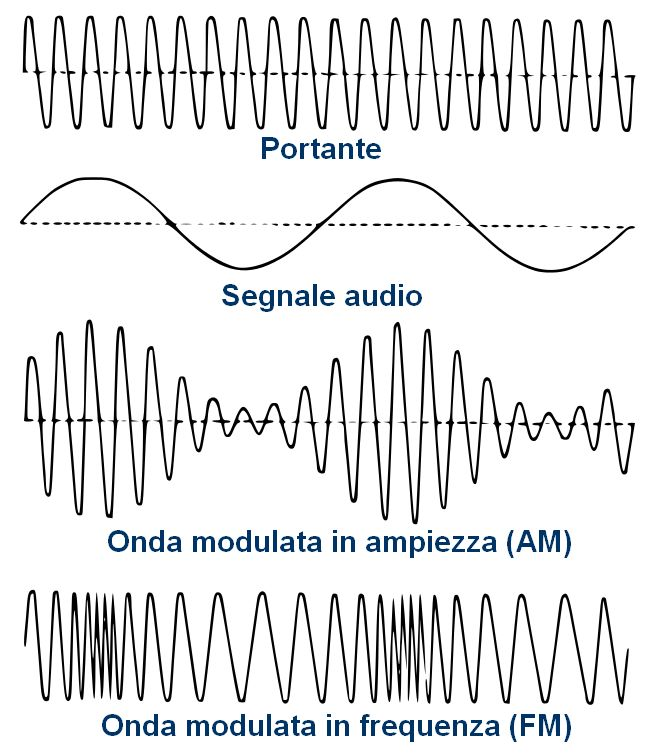
\includegraphics[scale=0.3]{amfm}
  \begin{figure}[h]
  	\centering
  	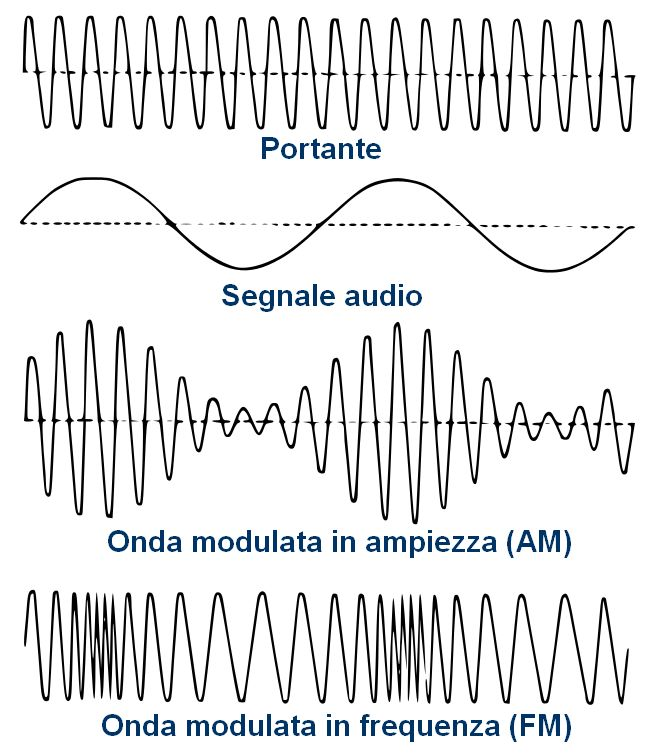
\includegraphics[scale=0.3]{amfm}
  	\caption{rappresentazione segnale modulato am e fm nel tempo}\label{fig:1}
  \end{figure}


\section{Modulazioni Digitali}
\label{sec:context}
\begin{itemize}
  \item \subsection{FSK (frequency shifting key): } questa tecnica di modulazione codifica l' informazione variando la frequenza della portante in valori predefiniti, ad esempio per ottenere una codifica binaria alterna due frequenze diverse. Questa tecnica ha il vantaggio di essere facile nell'implementazione e poco soggetta ad interferenze tuttavia necessita di una maggiore larghezza di banda rispetto ad altre modulazioni digitali quali psk o ask.
  \cite{fsk}
  \item \subsection{ASK (Amplitude shift keying): } la modulazione viene effettuata variando l' ampiezza del segnale portante alzandola o abbassandola in relazione alle informazioni da trasmettere, richiede un canale più affidabile in grado di ricevere anche i livelli di ampiezza più bassi. Trova ancora utilizzo nelle fibre ottiche e viene tuttora utilizzata la sua versione a codifica binaria (solo due livelli di potenza della portante presente/non presente) che prende il nome di OOF(on/off keying) in passato utilizzata anche per trasmettere messaggi in codice morse.
  \cite{ask}
  \item \subsection{PSK (Phase Shift Keying): } questo tipo di modulazione codifica le informazioni in ingresso variando la fase della portante, ne esistono varie versioni che differiscono per il numero di valori diversi. La versione più semplice è la binaryPSK che varia di metà periodo mentre versioni come la 4PSK di un quarto e così via per la variante 8PSK e 16PSK. Tali possibili sfasature della portante vengono dette costellazione e vengono di norma rappresentate come coordinate complesse su un grafico. Sulle ascisse si trova la portante mentre sulle ordinate si trova in quadratura ovvero sfasata di 90°.La lunghezza del vettore fra l'origine e uno dei punti della costellazione rappresenta l' ampiezza del segnale modulato mentre l'angolo rappresenta la sfasatura rispetto alla portante. Esiste una variante di 4PSK detta QPSK che differisce per una disposizione della costellazione ruotata di 45°.
  \begin{figure}[h]
  	\centering
  	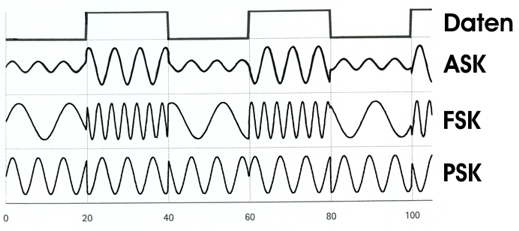
\includegraphics[scale=2.0]{digital}
  	\caption{rappresentazione segnale modulato nel tempo ASK FSK e PSK \cite{digit}}\label{fig:1}
  \end{figure}
  \item \subsection{DPSK (Differential Phase Shift Keying): } questa tecnica differisce da PSK solo per la particolarità di codificare il simbolo non utilizzando una costellazione fissa, le informazioni sono espresse come cambio di fase rispetto al simbolo precedente. Tale caratteristica rende questa modulazione robusta sia contro variazioni di ampiezza come psk sia contro distorsioni della fase del segnale ricevuto.
  \begin{figure}[h]
  	\centering
  	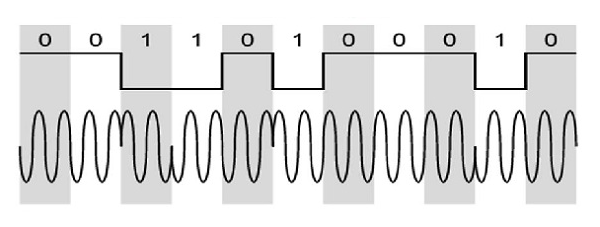
\includegraphics[scale=0.6]{dpsk}
  	\caption{rappresentazione segnale modulato DPSK \cite{dpsk}}\label{fig:1}
  \end{figure}
    
  \item \subsection{QAM (Quadrature amplitude modulation): } è una tecnica di modulazione simile a psk ma introduce la modulazione anche in ampiezza. La costellazione risulta avere punti non più equidistanti dall' origine. QAM come PSK presenta varianti che differiscono per il numero di punti sulla costellazione, in sistemi moderni si utilizzano anche 256 punti. Una particolarità comune a psk consiste nel fatto che due punti della costellazione adiacente differiscono per un solo bit, ciò incrementa l' efficacia di un eventuale error recovery. QAM viene anche utilizzato per trasferire più flussi analogici contemporaneamente, questo particolare utilizzo fa si che QAM venga considerato anche come una tecnica di modulazione analogica. 
  \cite{qam}
  
  \begin{figure}[h]
	\centering
	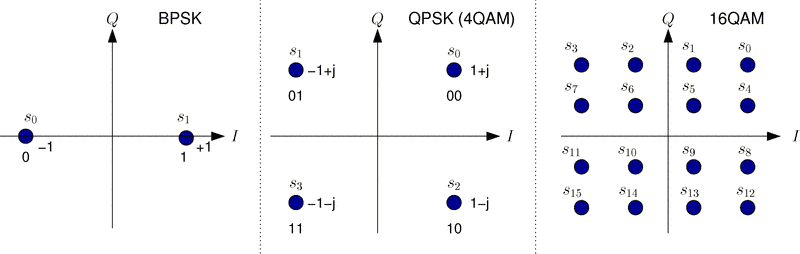
\includegraphics[scale=1.5]{constellation}
	\caption{Costellazioni BPSK, QPSK(4QAM), 16PSK \cite{psk-constellation}}\label{fig:1}
  \end{figure} 
  \end{itemize}
  %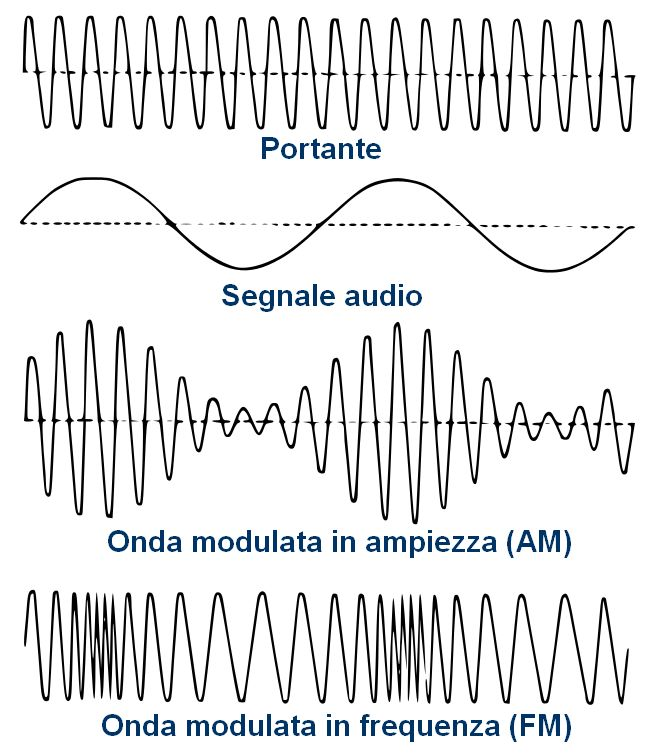
\includegraphics[scale=0.3]{amfm}


\section{OFDM (orthogonal frequency-division multiplexing): }
OFDM è una tecnica di codifica digitale su portanti multiple, su ogni sotto portante vengono modulate le informazioni utilizzando una delle varie tecniche digitali disponibili (solitamente si utilizza una versione di PSK oppure di QAM). OFSM trova svariati utilizzi nei sistemi di comunicazione moderni come ad esempio adsl, fibra ottica, 4G, wi-fi(802.11a/g/n/ac), radio/televisione digitale e WiMAX.
\cite{ofdm}
\cite{ofdm2}

\label{sec:problem}
\subsection{Principi di funzionamento}
\begin{itemize}
	 \item \textbf{ortogonalità delle sottoportanti: } la divisione della larghezza di banda disponibile in sezioni più piccole non è una caratteristica unica di OFDM, ciò che lo distingue è la soluzione al problema di interferenza fra i sotto canali. La soluzione classica è quella di lasciare delle piccole bande di frequenza vuote dove non si trasmette fra un canale e quello adiacente, da notare che in questo tipo di approccio si ha una allocazione inefficiente della larghezza di banda disponibile. OFDM utilizza la proprietà di ortogonalità per riuscire addirittura a sovrapporre perzialmente un canale con il successivo evitando sprechi di banda e aumentando così l' efficienza spettrale ( indica la bontà del sistema nello sfruttare in maniera più o meno efficiente la banda disponibile \cite{efficienzaSpettrale}).
	 La spiegazione matematica di questa tecnica è complessa e fa uso della trasformata di Fourier, è tuttavia possibile intuirne il funzionamento dall' immagine sottostante. L'immagine rappresenta la disposizione delle sotto portanti, sulle ascisse troviamo le frequenze mentre sulle ordinate l'ampiezza. Ogni picco rappresenta la presenza di un simbolo modulato sulla rispettiva portante. E' possibile notare che in questa particolare disposizione il rumore che genererebbe ogni canale all'esterno della propria banda si annulla esattamente in corrispondenza delle frequenze di trasmissione dei simboli adiacenti non creandogli disturbo. Perchè l'ortogonalità garantisca che non ci siano interferenze fra le diverse sottoportanti è necessario che il tempo di trasmissione dei simboli sia uguale in tutto il sistema, in ambienti caratterizzati da una variazione dell' attenuazione sul mezzo trasmissivo ad esempio sul doppino adsl un eventuale algoritmo finalizzato ad aumentare il throughput non potrà agire sulla velocità di trasmissione dei simboli ma sulla grandezza della costellazione utilizzata per modulare nella sottoportante (passando ad esempio da un bpsk che trasferisce un bit per simbolo a 16psk che ne trasferisce 4)). Altro requisito fondamentale che verrà ripreso nella sezione dedicata all'implementazione sul software gnuradio è la necessità di avere un ottima sincronizzazione sulla frequenza fra trasmettitore e ricevitore, le cause di una cattiva sincronizzazione possono essere varie un esempio è l'effetto Doppler causato dal movimento di un apparato rispetto all' altro durante la comunicazione, il cosiddetto multi-path per le reti wireless oppure semplici imperfezioni sul clock (generatore di frequenza) fra gli apparati.
	 \begin{figure}[h]
	 	\centering
		\begin{minipage}[b]{.5\columnwidth}
	 		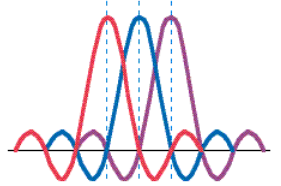
\includegraphics[scale=0.9]{ofdm-simboli}
	 		\caption{ortogonalità sottoportanti OFDM \cite{ofdm-simboli}}\label{fig:1}
 		\end{minipage}\hfill
 		\begin{minipage}[b]{.5\columnwidth}
 			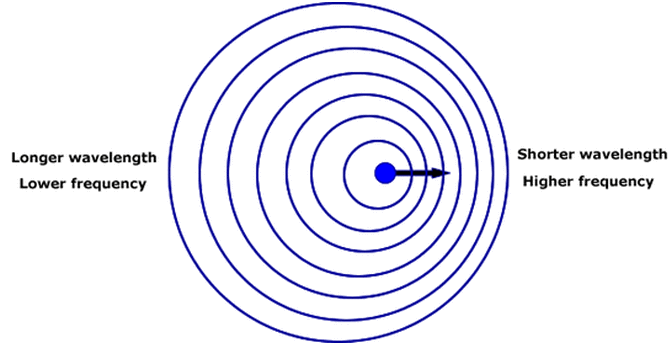
\includegraphics[scale=0.3]{doppler}
 			\caption{effetto Doppler \cite{doppler}}\label{fig:1}
 		\end{minipage}\hfill
 	\end{figure}
 	 \item \textbf{tempi di guardia } OFDM può soffrire di ISI(intersymbol interference) per uno dei problemi appena esposti nella sezione precedente. Questo problema avviene quando un simbolo trasmesso arriva al ricevitore assieme al precedente facendo fallire la decodifica, per risolvere questo problema viene aggiunto un tempo detto di guardia lungo solitamente attorno ad 1/10 del simbolo. Inizialmente durante questo breve intervallo non veniva trasmesso nulla, successivamente è risultato più efficiente trasmette l' ultimo pezzo del simbolo dopo (cyclic prefix) favorendo la corretta decodifica  ricevitore.
 	 \begin{figure}[h]
 	 	\centering
 	 	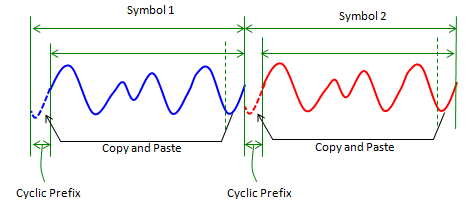
\includegraphics[scale=1]{cp}
 	 	\caption{cyclic guard \cite{cp}}\label{fig:1}
 	 \end{figure}
     \item \textbf{equalizzazione} l'equalizzazione del segnale ricevuto è una procedura fondamentale per la corretta decodifica delle informazioni. L'obiettivo di questa procedura è quello di modificare il segnale ricevuto cercando di agire esattamente nel modo opposto di come è stato distorto dal canale in modo da annullarne la distorsione, per ottenere tale risultato esistono numerosi algoritmi di equalizzazione che differiscono per gli approcci diversi in relazione alle informazioni disponibili sul mezzo trasmissivo oppure alle informazioni ottenute durante la trasmissione stessa. Esistono due tipi di equalizzazione possibile uno nel dominio del tempo quindi analizzando lo scorrere dei simboli e uno nel dominio delle frequenze che analizza il comportamento del canale nelle varie sottoportanti. All'inizio di una trasmissione OFDM vengono inviati dei simboli pilota ben noti al ricevitore che li utilizza per stimare la distorsione del canale di trasmissione, il ricevitore aggiusta le proprie previsioni anche mentre sta ricevendo grazie al preambolo contenuto nei pacchetti. Da notare che l'equalizzatore assieme al segnale aumenta anche il rumore.
     \begin{figure}[h]
     	\centering
     	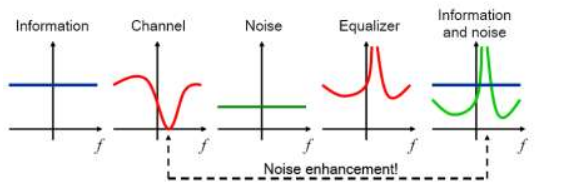
\includegraphics[scale=0.7]{equalizer}
     	\caption{principio funzionamento equalizzatore \cite{equalizer}}\label{fig:1}
     \end{figure}
 \item \textbf{recupero degli errori} Individuare e correggere gli errori avvenuti nella trasmissione è un compito complesso. OFDM solitamente utilizza CC (Convolutional coding) per la deteminazione e la correzione dell' errore, il principio di funzionamento di questo algoritmo si basa sulla creazione di un diagramma a stati che permette di codificare non solo la sequenza di bit in ingresso ma anche la loro transizione di stato. Il rapporto fra quantità di bit in ingresso e quello in uscita è detto code rate e può variare a seconda delle ciscostanze, un code rate di 1/2 ad esempio aggiunge 1 bit ogni bit in ingresso mentre con un rapporto 4/5 viene aggiunto un bit ogni 4. Meno bit aggiunti si traduce in meno bit da inviare ma minore efficacia nella correzione d'errore.
 \cite{cc}
	 \begin{figure}[h]
	 	\centering
	 	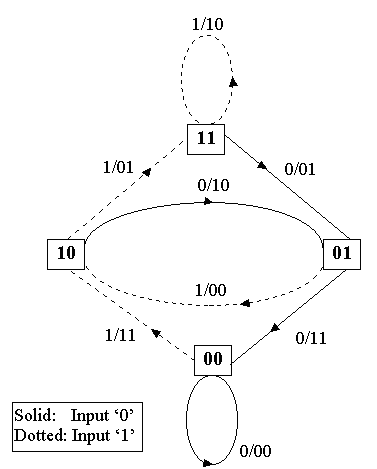
\includegraphics[scale=0.4]{ccDiagram}
	 	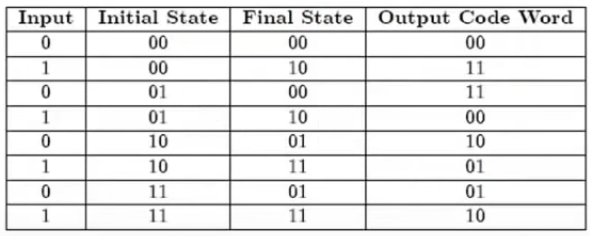
\includegraphics[scale=0.4]{ccTable}
	 	\caption{diagramma a stati e tabella utilizzati per un implementazione di un codificatore CC con output di lunghezza doppia rispetto all'input.}\label{fig:1}
	 \end{figure}
 Spesso in OFDM la tecnica di Convolutional coding viene utilizzata assieme ad altre tecniche di recupero errore più complesse come ad esempio Reed-Solomon in grado di recuperare ulteriormente informazioni danneggiate.
 E' bene puntualizzare che esiste un limite matematicamente dimostrato insuperabile alla quantità di informazioni trasferibili su un canale affetto da rumore, questo limite è detto di Shannon.
 \cite{ofdmWiki}
\label{sec:problem}
\subsection{Proprietà e campi di utilizzo}
OFDM grazie all'ortogonalità delle portanti permette di avere un ottima efficienza sull'utilizzo della banda, inoltre la scelta statica o dinamica del tipo di modulazione da utilizzare in ogni sottoportante lo rende adatto sia in situazioni dove è presente un canale molto distorcente che in casi in cui è possibile raggiungere un elevato throughput. Grazie ai tempi di guardia fra i simboli trasmessi e al prefisso ciclico (Cyclic prefix) OFDM risulta robusto contro il problema della sovrapposizione sul segnale in ricezione di componenti provenienti da segnali riflessi (multipath propagation). OFDM richiede un ottima sincronizzazione e risulta quindi sensibile all'effetto Doppler. OFDM soffre inoltre di un elevato PAPR (peak to average power ratio) causato dalla caratteristica di avere le sottoportanti in quadratura. L'ortogonalità garantisce di non avere sovrapposizioni sulla frequenza dove si trasmette un simbolo ma ciò non si verifica nelle frequenze intermedie fra una sottoportante e l'adiacente. Accade così che in particolari circostanze le sfasature fra i simboli su sottoportanti adiacenti finiscano per sommarsi creando un picco ben superiore alla media. Questo fenomeno influisce nel dimensionamento degli apparati che devono essere scelti per non saturare il segnale ma allo stesso tempo che non siano sprecati funzionando sotto alla metà della potenza.
\cite{papr}
\begin{itemize}
	\item \textbf{ADSL} la connessione adsl avviene mediante doppini lunghi anche qualche chilometro. Il doppino di rame presenta fisicamente una resistenza (prevedibile con la seconda legge di ohm) che è posizionata in serie al segnale, inoltre il doppino possiede un induttanza. Quando è presente un segnale (corrente alternata) si comporta come un filtro che attenua il segnale, tali effetti si amplificano all'aumentare della distanza e della frequenza. OFDM viene utilizzato in questo campo proprio perchè non risente molto della differenza di attenuazione nelle sottoparti del canale trasmissivo.
\end{itemize}
\begin{itemize}
	\item \textbf{Powerline} i dispositivi powerline uitilizzano l'impianto elettrico come mezzo trasmissivo, viene utilizzato OFDM per la presenza di un canale molto variabile e soggetto da disturbi esterni non prevedibili.
\end{itemize}
\begin{itemize}
	\item \textbf{Wlan, WiMAX}
	  OFDM viene utilizzato in due fra i principali standard per la trasmissione di internet senza fili. fornisce robustezza contro il problema della multipath propagation oltre ad un ottimo range di scelta sulle modulazioni che si presta bene sia per situazioni di bassa qualità del canale sia in situazioni di stabilità dove si vuole ottenere un buon bandwidht.
\end{itemize}
\begin{itemize}
	\item \textbf{Radio e televisione digitali} La televisione pubblica italiana come molte di quelle europee vengono trasmesse secondo lo standard DVB-T(Digital Video Broadcasting-Terrestrial) che sfrutta OFDM per inviare un flusso contenente i vari canali televisivi già compressi e provvisti di trame per la decodifica. La radio digitale DAB(Digital Audio Broadcasting) suddivide invece le stazioni in blocchi contenenti una decina di radio ognuno. Ogni blocco viene poi trasmesso utilizzando OFDM
\end{itemize}

\section{SDR (Software Defined Radio)} Tradizionalmente gli apparati per le telecomunicazioni vengono implementati in hardware, lo sviluppo risulta molto costoso finendo per essere svolto da poche persone. Progettare in hardware richiede molto tempo ed il risultato è un sistema affidabile ma con un compito specifico e difficile da aggiornare o modificare una volta prodotto. Recentemente con l'aumento della potenza di calcolo è finalmente possibile svolgere con il software compiti precedentemente svolti da hardware specializzato. L'SDR è una scheda che contiene l'hardware aggiuntivo necessario ad un computer per poter ricevere e/o trasmettere informazioni. Un grande vantaggio dell' utilizzo di queste piattaforme è la possibilità di implementare la tecnica di trasmissione favorita con inoltre la possibilità di variare tutti i parametri tecnici (es. frequenza, larghezza di banda, frequenza di campionamento, ecc.). Un applicazione interessante di questa tecnologia è la creazione di un sistema dinamico in grado di far variare la frequenza ed il metodo di trasmissione per adattarsi alla situazione presente nel migliore dei modi. Esistono diverse tipologie di SDR, i più economici costano appena una decina di euro e seppure con qualche limitazione riescono a ricevere fino a quasi 2GHZ, versioni più costose sono in grado anche di trasmettere contemporaneamente su un range di frequenza e sample rate più elevati. Da sottolineare che ogni diversa frequenza su cui si intende trasmettere-ricevere richiede una specifica antenna e che non esiste un antenna generica.
\begin{figure}[h]
	\centering
	\begin{minipage}[b]{.5\columnwidth}
		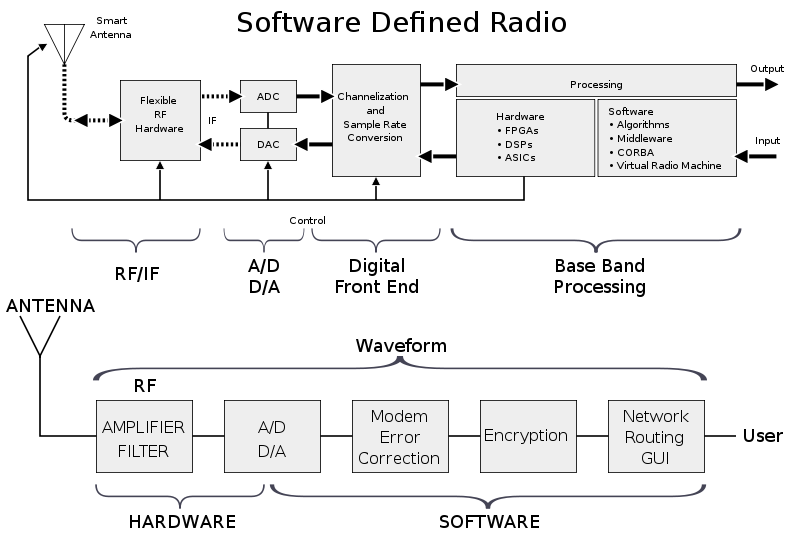
\includegraphics[scale=0.33]{sdrDiagram}
		\caption{Diagramma blocchi funzionamento SDR \cite{sdrDiagram}}\label{fig:1}
	\end{minipage}\hfill
	\begin{minipage}[b]{.4\columnwidth}
		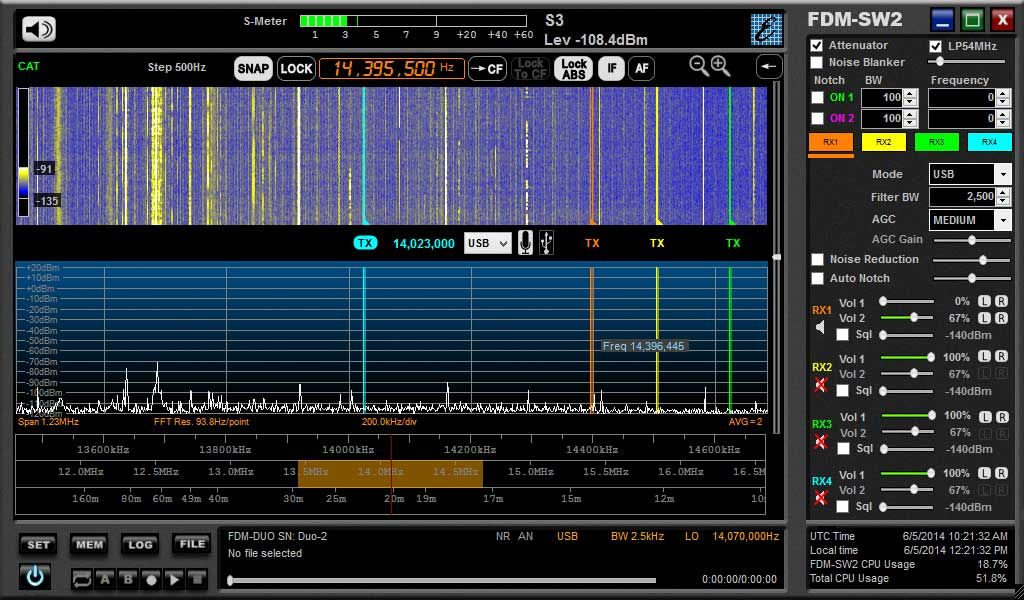
\includegraphics[scale=0.2]{sdrSoftware}
		\caption{Software generico per l analisi dello spettro \cite{sdrSoftware}}\label{fig:1}
	\end{minipage}\hfill
\end{figure}


\newpage